% questions.tex —— 2016 年·天津卷·理科 · 题目内容片段（无答案）
% 由 tools/generate_projects.py 依来源总账自 2016/2016_数学真题_天津理_试题.md 生成，勿手改（改源 MD 后重跑）


\gkpart{数学}

\begin{gktip}
\textbf{来源说明}：本题面依据固定源 PDF 两页 A3 页面逐题核对，原卷印刷页码 1023–1024。固定源不附答案；本文件仅为题面规范源。
\end{gktip}

\gkpart{一、选择题}

\begin{question}
\gkti{1}已知集合 \(A=\{1,2,3,4\}\)，\(B=\{y\mid y=3x-2,x\in A\}\)，则 \(A\cap B=\)（　）

（A）\(\{1\}\)　（B）\(\{4\}\)　（C）\(\{1,3\}\)　（D）\(\{1,4\}\)

\end{question}
\begin{question}
\gkti{2}设变量 \(x,y\) 满足约束条件

\nopagebreak[4]
\[
\begin{cases}
x-y+2\geqslant 0,\\
2x+3y-6\geqslant 0,\\
3x+2y-9\leqslant 0,
\end{cases}
\]

则目标函数 \(z=2x+5y\) 的最小值为（　）

（A）\(-4\)　（B）\(6\)　（C）\(10\)　（D）\(17\)

\end{question}
\begin{question}
\gkti{3}在 \(\triangle ABC\) 中，若 \(AB=\sqrt{13}\)，\(BC=3\)，\(\angle C=120^{\circ}\)，则 \(AC=\)（　）

（A）\(1\)　（B）\(2\)　（C）\(3\)　（D）\(4\)

\Needspace{0.48\textheight}

\Needspace{0.4\textheight}
\end{question}
\begin{question}
\gkti{4}阅读如下的程序框图，运行相应的程序，则输出 \(S\) 的值为（　）
\nopagebreak[4]
\begin{center}% 第 4 题程序框图（累减计数型，双菱形双汇入结构）：按固定源 PDF 逐框重绘（10 框；1 pt → 0.04 cm）。
% 结构要点（易错，矢量路径逐段核对）：
%   主干 x=0（两个菱形与主线上全部处理框同一中心线）；左支 x=-2.45（S=2S）；右回线 x=+2.34。
%   第一菱形「否」自左顶点向左折下入 S=2S，其回接自框底垂直下、水平右，汇入主干 y=4.87
%   （S=S-6 之后、n=n+1 之前）；第二菱形「否」自右顶点向右、向上至 y=7.45、向左汇入主干
%   （n=1 之后、第一菱形之前）。两处汇入高度不同，均不做自环。
%   全图 11 个箭头；输出框为向右倾平行四边形；无输入框。
\begin{tikzpicture}[>=stealth,every node/.style={font=\small},
  term/.style={draw,rounded corners,minimum width=1.5cm,minimum height=5.5mm},
  box/.style={draw,minimum height=5.5mm,inner xsep=4pt},
  io/.style={draw,trapezium,trapezium left angle=70,trapezium right angle=110,minimum width=1.8cm,minimum height=5.5mm},
  decision/.style={draw,diamond,aspect=4,minimum width=3.2cm,inner sep=0pt}]
\node[term] (start) at (0,10.36) {开始};
\node[box] (s4) at (0,9.16) {\(S=4\)};
\node[box] (n1) at (0,8.02) {\(n=1\)};
\node[decision] (t1) at (0,6.75) {\(S\geqslant 6?\)};
\node[box] (s6) at (0,5.46) {\(S=S-6\)};
\node[box] (s2s) at (-2.45,5.46) {\(S=2S\)};
\node[box] (np1) at (0,4.28) {\(n=n+1\)};
\node[decision] (t2) at (0,3.03) {\(n>3?\)};
\node[io] (out) at (0,1.74) {输出 \(S\)};
\node[term] (end) at (0,0.46) {结束};
\draw[->] (start)--(s4);
\draw[->] (s4)--(n1);
\draw[->] (n1)--(t1);
\draw[->] (t1.south)--(s6.north);
\draw[->] (s6)--(np1);
\draw[->] (np1)--(t2);
\draw[->] (t2.south)--(out.north);
\draw[->] (out)--(end);
% 第一菱形「否」：左顶点向左折下入 S=2S
\draw[->] (t1.west) -| (s2s.north);
% S=2S 回接：框底垂直向下、水平向右汇入主干（汇入点高于 n=n+1）
\draw[->] (s2s.south) |- (0,4.87);
% 第二菱形「否」：右顶点向右、向上、向左汇入主干（汇入点高于第一菱形）
\draw[->] (t2.east) -- (2.34,3.03) -- (2.34,7.45) -- (0,7.45);
% 分支标注（「否」在各自水平线上方、「是」在主干竖线右侧）
\node at (-1.64,7.05) {否};
\node at (0.65,6.15) {是};
\node at (1.55,3.38) {否};
\node at (0.65,2.42) {是};
\end{tikzpicture}
\end{center}
\nopagebreak[4]
（A）\(2\)　（B）\(4\)　（C）\(6\)　（D）\(8\)

\end{question}
\begin{question}
\gkti{5}设 \(\{a_{n}\}\) 是首项为正数的等比数列，公比为 \(q\)，则“\(q<0\)”是“对任意的正整数 \(n\)，\(a_{2n-1}+a_{2n}<0\)”的（　）

（A）充要条件　（B）充分而不必要条件

（C）必要而不充分条件　（D）既不充分也不必要条件

\end{question}
\begin{question}
\gkti{6}已知双曲线 \(\dfrac{x^{2}}{4}-\dfrac{y^{2}}{b^{2}}=1\)（\(b>0\)），以原点为圆心，双曲线的实半轴长为半径长的圆与双曲线的两条渐近线相交于 \(A,B,C,D\) 四点，四边形 \(ABCD\) 的面积为 \(2b\)，则双曲线的方程为（　）

（A）\(\dfrac{x^{2}}{4}-\dfrac{3y^{2}}{4}=1\)　（B）\(\dfrac{x^{2}}{4}-\dfrac{4y^{2}}{3}=1\)　（C）\(\dfrac{x^{2}}{4}-\dfrac{y^{2}}{4}=1\)　（D）\(\dfrac{x^{2}}{4}-\dfrac{y^{2}}{12}=1\)

\end{question}
\begin{question}
\gkti{7}已知 \(\triangle ABC\) 是边长为 \(1\) 的等边三角形，点 \(D,E\) 分别是边 \(AB,BC\) 的中点，连接 \(DE\) 并延长到点 \(F\)，使得 \(DE=2EF\)，则 \(\overrightarrow{AF}\cdot\overrightarrow{BC}\) 的值为（　）

（A）\(-\dfrac{8}{5}\)　（B）\(\dfrac{1}{8}\)　（C）\(\dfrac{1}{4}\)　（D）\(\dfrac{11}{8}\)

\Needspace{0.49\textheight}

\end{question}
\begin{question}
\gkti{8}已知函数

\nopagebreak[4]
\[
f(x)=\begin{cases}
x^{2}+(4a-3)x+3a, & x<0,\\
\log_{a}(x+1)+1, & x\geqslant 0,
\end{cases}
\]

（\(a>0\)，且 \(a\neq 1\)）在 \(\mathbf{R}\) 上单调递减，且关于 \(x\) 的方程 \(|f(x)|=2-x\) 恰好有两个不相等的实数解，则 \(a\) 的取值范围是（　）

（A）\(\left(0,\dfrac{2}{3}\right]\)　（B）\(\left[\dfrac{2}{3},\dfrac{3}{4}\right]\)

（C）\(\left[\dfrac{1}{3},\dfrac{2}{3}\right]\cup\left\{\dfrac{3}{4}\right\}\)　（D）\(\left[\dfrac{1}{3},\dfrac{2}{3}\right)\cup\left\{\dfrac{3}{4}\right\}\)

\end{question}
\gkpart{二、填空题}

\begin{question}
\gkti{9}已知 \(a,b\in\mathbf{R}\)，\(\mathrm{i}\) 是虚数单位，若 \((1+\mathrm{i})(1-b\mathrm{i})=a\)，则 \(\dfrac{a}{b}\) 的值为 \(\underline{\qquad}\)。

\end{question}
\begin{question}
\gkti{10}\(\left(x^{2}-\dfrac{1}{x}\right)^{8}\) 的展开式中 \(x^{7}\) 的系数为 \(\underline{\qquad}\)。（用数字作答）

\Needspace{0.4\textheight}
\end{question}
\begin{question}
\gkti{11}已知一个四棱锥的底面是平行四边形，该四棱锥的三视图如图所示（单位：m），则该四棱锥的体积为 \(\underline{\qquad}\) \(\mathrm{m}^{3}\)。
\nopagebreak[4]
\begin{center}% 第 11 题四棱锥三视图：正视图（左上，等腰三角形＋内部实线/虚线/各连向顶点）、侧视图（右上，
% 等腰三角形无内部线）、俯视图（左下，平行四边形＋两条对角线）。按固定源 PDF 矢量坐标换算，
% 单位 u = 25.5 pt = 0.896 cm（原图 1 m 按 25.5 pt 绘制）；坐标以正视图底边左端为原点、y 向上。
% 尺寸标注：左侧竖直「3」尺寸线（两端外向箭头、上下端线向左伸）、底边下方水平尺寸链
% 「1+1+1」与侧视图「1」（各被数字断开、6 条竖直端线）；三段图注居中于各自图形下方。
\begin{tikzpicture}[>=stealth,x=0.896cm,y=0.896cm,every node/.style={font=\small}]
% ===== 正视图 =====
\draw (0,0)--(3,0)--(1.5,3)--cycle;
\draw (2,0)--(1.5,3);
\draw[dashed] (1,0)--(1.5,3);
% 左侧竖直尺寸线（x = -0.3），两端外向箭头，数字 3
\draw[->] (-0.3,0.55)--(-0.3,0);
\draw[->] (-0.3,2.45)--(-0.3,3);
\node at (-0.3,1.5) {\(3\)};
\draw (-0.5,3)--(-0.1,3);
\draw (-0.5,0)--(-0.1,0);
% 底边下方水平尺寸链（y = -0.3）：三段 1
\draw[->] (0.45,-0.3)--(0,-0.3);
\draw[->] (0.55,-0.3)--(1,-0.3);
\node at (0.5,-0.3) {\(1\)};
\draw[->] (1.45,-0.3)--(1,-0.3);
\draw[->] (1.55,-0.3)--(2,-0.3);
\node at (1.5,-0.3) {\(1\)};
\draw[->] (2.45,-0.3)--(2,-0.3);
\draw[->] (2.55,-0.3)--(3,-0.3);
\node at (2.5,-0.3) {\(1\)};
\draw (0,-0.5)--(0,-0.1);
\draw (1,-0.5)--(1,-0.1);
\draw (2,-0.5)--(2,-0.1);
\draw (3,-0.5)--(3,-0.1);
\node[anchor=north] at (1.5,-0.77) {正视图};
% ===== 侧视图（与正视图同基线）=====
\draw (4,0)--(5,0)--(4.5,3)--cycle;
\draw[->] (4.45,-0.3)--(4,-0.3);
\draw[->] (4.55,-0.3)--(5,-0.3);
\node at (4.5,-0.3) {\(1\)};
\draw (4,-0.5)--(4,-0.1);
\draw (5,-0.5)--(5,-0.1);
\node[anchor=north] at (4.5,-0.77) {侧视图};
% ===== 俯视图（正视图正下方）=====
\draw (0,-2.5)--(2,-2.5)--(3,-1.5)--(1,-1.5)--cycle;
\draw (0,-2.5)--(3,-1.5);
\draw (2,-2.5)--(1,-1.5);
\node[anchor=north] at (1.5,-2.77) {俯视图};
\end{tikzpicture}
\end{center}
\nopagebreak[4]
\Needspace{0.4\textheight}
\end{question}
\begin{question}
\gkti{12}如图，\(AB\) 是圆的直径，弦 \(CD\) 与 \(AB\) 相交于点 \(E\)，\(BE=2AE=2\)，\(BD=ED\)，则线段 \(CE\) 的长为 \(\underline{\qquad}\)。
\nopagebreak[4]
\begin{center}% 第 12 题圆：按固定源 PDF 矢量路径换算（1 pt → 0.03515 cm），取圆心为原点、y 向上。
% 圆心 (594.74,610.27) pt、半径 40.08 pt；直径 AB 水平过圆心；弦 CD 自左上（C 在圆上）经 E（在 AB 上）
% 至右下（D 在圆上，BD=ED）；线段 BD。图中不标圆心、无直角标记、无长度数字。
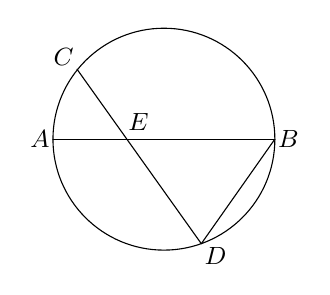
\begin{tikzpicture}[line cap=round,line join=round,font=\small]
\draw (0,0) circle (1.409);
\draw (-1.409,0)--(1.409,0);
\draw (-1.103,0.888)--(0.475,-1.327);
\draw (1.409,0)--(0.475,-1.327);
\node[above left,inner sep=1pt] at (-1.103,0.888) {$C$};
\node[left,inner sep=1pt] at (-1.409,0) {$A$};
\node at (-0.324,0.220) {$E$};
\node[right,inner sep=1pt] at (1.409,0) {$B$};
\node[below right,inner sep=1pt] at (0.475,-1.327) {$D$};
\end{tikzpicture}
\end{center}
\nopagebreak[4]
\end{question}
\begin{question}
\gkti{13}已知 \(f(x)\) 是定义在 \(\mathbf{R}\) 上的偶函数，且在区间 \((-\infty,0)\) 上单调递增。若实数 \(a\) 满足 \(f\left(2^{|a-1|}\right)>f\left(-\sqrt{2}\right)\)，则 \(a\) 的取值范围是 \(\underline{\qquad}\)。

\end{question}
\begin{question}
\gkti{14}设抛物线

\nopagebreak[4]
\[
\begin{cases}
x=2pt^{2},\\
y=2pt,
\end{cases}
\]

（\(t\) 为参数，\(p>0\)）的焦点为 \(F\)，准线为 \(l\)。过抛物线上一点 \(A\) 作 \(l\) 的垂线，垂足为 \(B\)。设 \(C\left(\dfrac{7}{2}p,0\right)\)，\(AF\) 与 \(BC\) 相交于点 \(E\)。若 \(|CF|=2|AF|\)，且 \(\triangle ACE\) 的面积为 \(3\sqrt{2}\)，则 \(p\) 的值为 \(\underline{\qquad}\)。

\end{question}
\gkpart{三、解答题}

\begin{question}
\gkti{15}已知函数 \(f(x)=4\tan x\sin\left(\dfrac{\pi}{2}-x\right)\cos\left(x-\dfrac{\pi}{3}\right)-\sqrt{3}\)。

（1） 求 \(f(x)\) 的定义域与最小正周期；

（2） 讨论 \(f(x)\) 在区间 \(\left[-\dfrac{\pi}{4},\dfrac{\pi}{4}\right]\) 上的单调性。

\end{question}
\begin{question}
\gkti{16}某小组共 \(10\) 人，利用假期参加义工活动，已知参加义工活动次数为 \(1,2,3\) 的人数分别为 \(3,3,4\)。现从这 \(10\) 人中随机选出 \(2\) 人作为该组代表参加座谈会。

（1） 设 \(A\) 为事件“选出的 \(2\) 人参加义工活动次数之和为 \(4\)”，求事件 \(A\) 发生的概率；

（2） 设 \(X\) 为选出的 \(2\) 人参加义工活动次数之差的绝对值，求随机变量 \(X\) 的分布列和数学期望。

\Needspace{0.4\textheight}
\end{question}
\begin{question}
\gkti{17}如图，正方形 \(ABCD\) 的中心为 \(O\)，四边形 \(OBEF\) 为矩形，平面 \(OBEF\perp\) 平面 \(ABCD\)，点 \(G\) 为 \(AB\) 的中点，\(AB=BE=2\)。
\nopagebreak[4]
\begin{center}% 第 17 题多面体 ABCDEF：按固定源 PDF 矢量路径端点换算（1 pt → 0.03515 cm；斜二测画法，
% x 水平实长、y 45° 半长、z 竖直实长）。以 B 为原点。
% 实线 7 条：EC、EF、FC、FA、FD、AD、DC；虚线 8 条：BE、EG（辅助）、EA、OF、BH（辅助）、BC、AB、BO。
% G 为 AB 中点（虚线连 E）；H 在 AF 上 AH:HF=2:3（虚线连 B）。先画虚线后画实线。
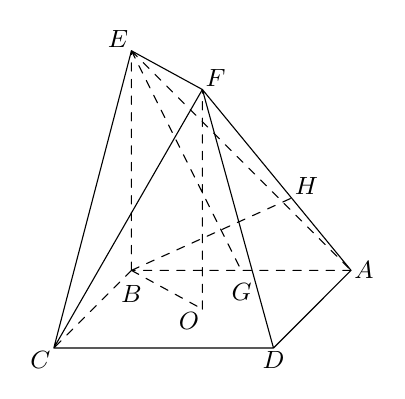
\begin{tikzpicture}[line cap=round,line join=round,font=\small]
\coordinate (B) at (0,0);
\coordinate (A) at (2.789,0);
\coordinate (C) at (-0.986,-0.986);
\coordinate (D) at (1.804,-0.986);
\coordinate (O) at (0.901,-0.492);
\coordinate (E) at (0,2.789);
\coordinate (F) at (0.901,2.297);
\coordinate (G) at (1.394,0);
\coordinate (H) at (2.034,0.919);
% 虚线先画
\draw[dashed] (B)--(E) (E)--(G) (E)--(A) (O)--(F) (B)--(H) (B)--(C) (A)--(B) (B)--(O);
% 实线后画
\draw (E)--(C) (E)--(F) (F)--(C) (F)--(A) (F)--(D) (A)--(D) (D)--(C);
\node[above left,inner sep=1pt] at (E) {$E$};
\node[above right,inner sep=1pt] at (F) {$F$};
\node[above right,inner sep=1pt] at (H) {$H$};
\node[right,inner sep=1pt] at (A) {$A$};
\node at (0,-0.30) {$B$};
\node at (1.399,-0.278) {$G$};
\node[below left,inner sep=1pt] at (O) {$O$};
\node[below left,inner sep=1pt] at (C) {$C$};
\node[below,inner sep=1pt] at (D) {$D$};
\end{tikzpicture}
\end{center}
\nopagebreak[4]
（1） 求证：\(EG\parallel\) 平面 \(ADF\)；

（2） 求二面角 \(O-EF-C\) 的正弦值；

（3） 设 \(H\) 为线段 \(AF\) 上的点，且 \(AH=\dfrac{2}{3}HF\)，求直线 \(BH\) 和平面 \(CEF\) 所成角的正弦值。

\Needspace{0.48\textheight}

\end{question}
\begin{question}
\gkti{18}已知 \(\{a_{n}\}\) 是各项均为正数的等差数列，公差为 \(d\)，对任意的 \(n\in\mathbf{N}^{*}\)，\(b_{n}\) 是 \(a_{n}\) 和 \(a_{n+1}\) 的等比中项。

（1） 设 \(c_{n}=b_{n+1}^{2}-b_{n}^{2}\)，\(n\in\mathbf{N}^{*}\)，求证：数列 \(\{c_{n}\}\) 是等差数列；

（2） 设 \(a_{1}=d\)，\(T_{n}=\displaystyle\sum_{k=1}^{2n}(-1)^{k}b_{k}^{2}\)，\(n\in\mathbf{N}^{*}\)，求证：\(\displaystyle\sum_{k=1}^{n}\dfrac{1}{T_{k}}<\dfrac{1}{2d^{2}}\)。

\end{question}
\begin{question}
\gkti{19}设椭圆 \(\dfrac{x^{2}}{a^{2}}+\dfrac{y^{2}}{3}=1\)（\(a>\sqrt{3}\)）的右焦点为 \(F\)，右顶点为 \(A\)。已知 \(\dfrac{1}{|OF|}+\dfrac{1}{|OA|}=\dfrac{3e}{|FA|}\)，其中 \(O\) 为原点，\(e\) 为椭圆的离心率。

（1） 求椭圆的方程；

（2） 设过点 \(A\) 的直线 \(l\) 与椭圆交于点 \(B\)（\(B\) 不在 \(x\) 轴上），垂直于 \(l\) 的直线与 \(l\) 交于点 \(M\)，与 \(y\) 轴交于点 \(H\)。若 \(BF\perp HF\)，且 \(\angle MOA\leqslant\angle MAO\)，求直线 \(l\) 的斜率的取值范围。

\end{question}
\begin{question}
\gkti{20}设函数 \(f(x)=(x-1)^{3}-ax-b\)，\(x\in\mathbf{R}\)，其中 \(a,b\in\mathbf{R}\)。

（1） 求 \(f(x)\) 的单调区间；

（2） 若 \(f(x)\) 存在极值点 \(x_{0}\)，且 \(f(x_{1})=f(x_{0})\)，其中 \(x_{1}\neq x_{0}\)，求证：\(x_{1}+2x_{0}=3\)；

（3） 设 \(a>0\)，函数 \(g(x)=|f(x)|\)，求证：\(g(x)\) 在区间 \([0,2]\) 上的最大值不小于 \(\dfrac{1}{4}\)。

\end{question}